% Created by tikzDevice version 0.10.1 on 2017-02-27 14:38:32
% !TEX encoding = UTF-8 Unicode
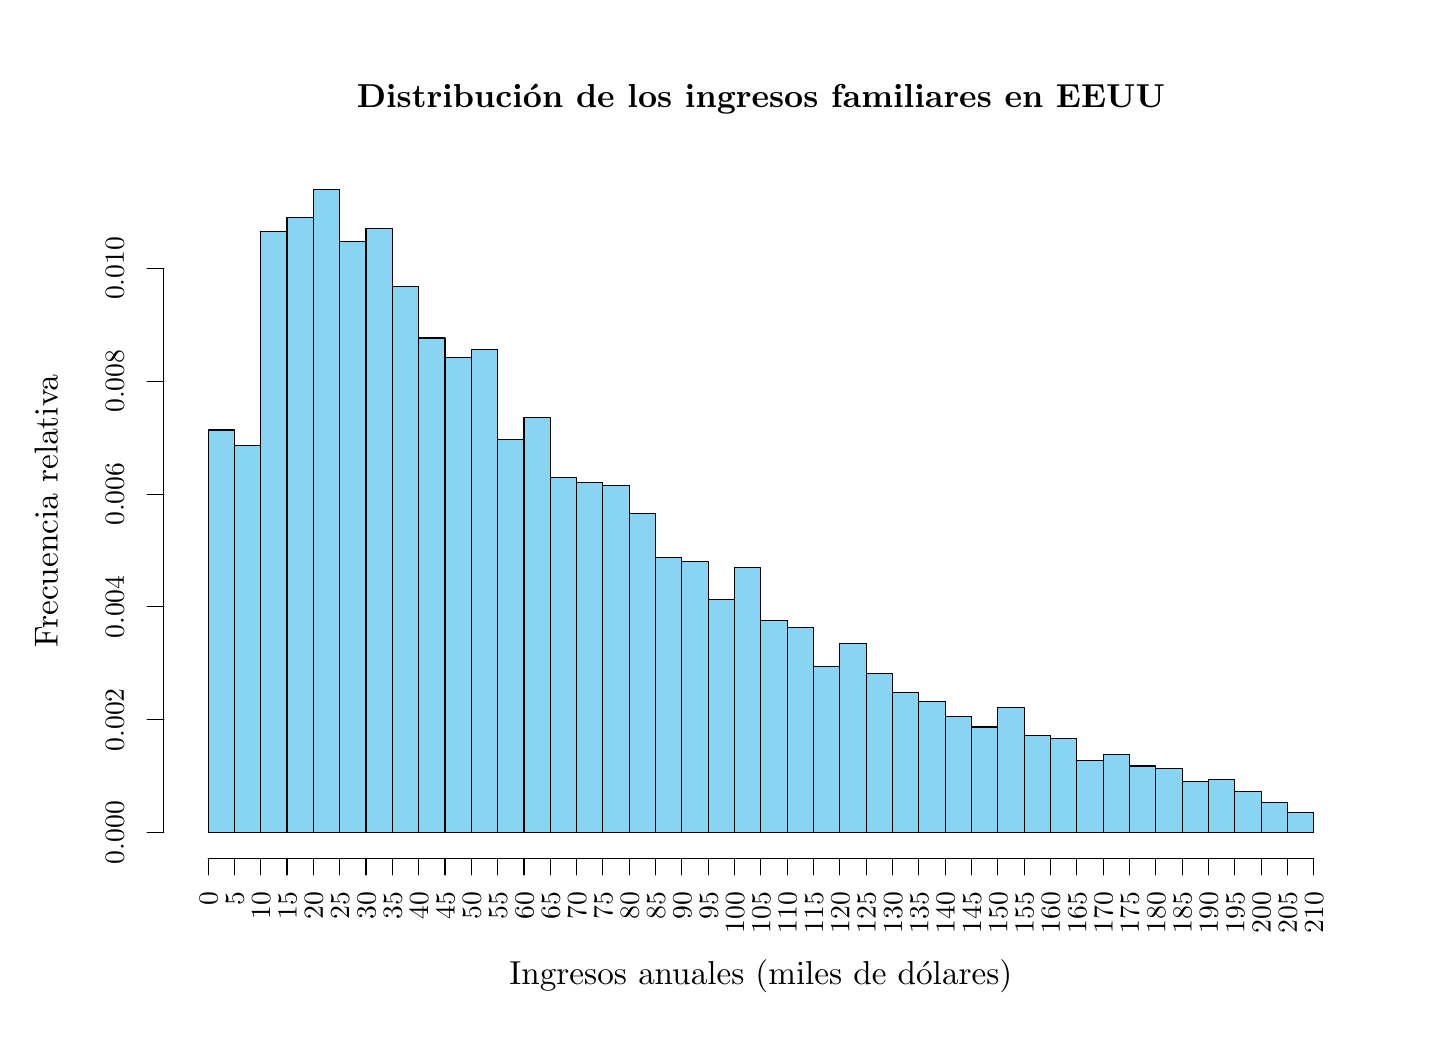
\begin{tikzpicture}[x=1pt,y=1pt]
\definecolor{fillColor}{RGB}{255,255,255}
\path[use as bounding box,fill=fillColor,fill opacity=0.00] (0,0) rectangle (505.89,361.35);
\begin{scope}
\path[clip] (  0.00,  0.00) rectangle (505.89,361.35);
\definecolor{drawColor}{RGB}{0,0,0}

\node[text=drawColor,anchor=base,inner sep=0pt, outer sep=0pt, scale=  1.20] at (264.94,332.61) {\bfseries Distribución de los ingresos familiares en EEUU};

\node[text=drawColor,anchor=base,inner sep=0pt, outer sep=0pt, scale=  1.20] at (264.94, 15.60) {Ingresos anuales (miles de dólares)};

\node[text=drawColor,rotate= 90.00,anchor=base,inner sep=0pt, outer sep=0pt, scale=  1.20] at ( 10.80,186.67) {Frecuencia relativa};
\end{scope}
\begin{scope}
\path[clip] (  0.00,  0.00) rectangle (505.89,361.35);
\definecolor{drawColor}{RGB}{0,0,0}

\path[draw=drawColor,line width= 0.4pt,line join=round,line cap=round] ( 49.20, 70.49) -- ( 49.20,274.36);

\path[draw=drawColor,line width= 0.4pt,line join=round,line cap=round] ( 49.20, 70.49) -- ( 43.20, 70.49);

\path[draw=drawColor,line width= 0.4pt,line join=round,line cap=round] ( 49.20,111.27) -- ( 43.20,111.27);

\path[draw=drawColor,line width= 0.4pt,line join=round,line cap=round] ( 49.20,152.04) -- ( 43.20,152.04);

\path[draw=drawColor,line width= 0.4pt,line join=round,line cap=round] ( 49.20,192.81) -- ( 43.20,192.81);

\path[draw=drawColor,line width= 0.4pt,line join=round,line cap=round] ( 49.20,233.58) -- ( 43.20,233.58);

\path[draw=drawColor,line width= 0.4pt,line join=round,line cap=round] ( 49.20,274.36) -- ( 43.20,274.36);

\node[text=drawColor,rotate= 90.00,anchor=base,inner sep=0pt, outer sep=0pt, scale=  1.00] at ( 34.80, 70.49) {0.000};

\node[text=drawColor,rotate= 90.00,anchor=base,inner sep=0pt, outer sep=0pt, scale=  1.00] at ( 34.80,111.27) {0.002};

\node[text=drawColor,rotate= 90.00,anchor=base,inner sep=0pt, outer sep=0pt, scale=  1.00] at ( 34.80,152.04) {0.004};

\node[text=drawColor,rotate= 90.00,anchor=base,inner sep=0pt, outer sep=0pt, scale=  1.00] at ( 34.80,192.81) {0.006};

\node[text=drawColor,rotate= 90.00,anchor=base,inner sep=0pt, outer sep=0pt, scale=  1.00] at ( 34.80,233.58) {0.008};

\node[text=drawColor,rotate= 90.00,anchor=base,inner sep=0pt, outer sep=0pt, scale=  1.00] at ( 34.80,274.36) {0.010};
\end{scope}
\begin{scope}
\path[clip] ( 49.20, 61.20) rectangle (480.69,312.15);
\definecolor{drawColor}{RGB}{0,0,0}
\definecolor{fillColor}{RGB}{137,211,243}

\path[draw=drawColor,line width= 0.4pt,line join=round,line cap=round,fill=fillColor] ( 65.18, 70.49) rectangle ( 74.69,215.96);

\path[draw=drawColor,line width= 0.4pt,line join=round,line cap=round,fill=fillColor] ( 74.69, 70.49) rectangle ( 84.21,210.32);

\path[draw=drawColor,line width= 0.4pt,line join=round,line cap=round,fill=fillColor] ( 84.21, 70.49) rectangle ( 93.72,287.71);

\path[draw=drawColor,line width= 0.4pt,line join=round,line cap=round,fill=fillColor] ( 93.72, 70.49) rectangle (103.23,292.72);

\path[draw=drawColor,line width= 0.4pt,line join=round,line cap=round,fill=fillColor] (103.23, 70.49) rectangle (112.74,302.86);

\path[draw=drawColor,line width= 0.4pt,line join=round,line cap=round,fill=fillColor] (112.74, 70.49) rectangle (122.26,284.20);

\path[draw=drawColor,line width= 0.4pt,line join=round,line cap=round,fill=fillColor] (122.26, 70.49) rectangle (131.77,288.74);

\path[draw=drawColor,line width= 0.4pt,line join=round,line cap=round,fill=fillColor] (131.77, 70.49) rectangle (141.28,267.75);

\path[draw=drawColor,line width= 0.4pt,line join=round,line cap=round,fill=fillColor] (141.28, 70.49) rectangle (150.79,249.20);

\path[draw=drawColor,line width= 0.4pt,line join=round,line cap=round,fill=fillColor] (150.79, 70.49) rectangle (160.31,242.30);

\path[draw=drawColor,line width= 0.4pt,line join=round,line cap=round,fill=fillColor] (160.31, 70.49) rectangle (169.82,244.91);

\path[draw=drawColor,line width= 0.4pt,line join=round,line cap=round,fill=fillColor] (169.82, 70.49) rectangle (179.33,212.69);

\path[draw=drawColor,line width= 0.4pt,line join=round,line cap=round,fill=fillColor] (179.33, 70.49) rectangle (188.84,220.49);

\path[draw=drawColor,line width= 0.4pt,line join=round,line cap=round,fill=fillColor] (188.84, 70.49) rectangle (198.36,198.71);

\path[draw=drawColor,line width= 0.4pt,line join=round,line cap=round,fill=fillColor] (198.36, 70.49) rectangle (207.87,197.00);

\path[draw=drawColor,line width= 0.4pt,line join=round,line cap=round,fill=fillColor] (207.87, 70.49) rectangle (217.38,195.86);

\path[draw=drawColor,line width= 0.4pt,line join=round,line cap=round,fill=fillColor] (217.38, 70.49) rectangle (226.89,185.70);

\path[draw=drawColor,line width= 0.4pt,line join=round,line cap=round,fill=fillColor] (226.89, 70.49) rectangle (236.41,169.86);

\path[draw=drawColor,line width= 0.4pt,line join=round,line cap=round,fill=fillColor] (236.41, 70.49) rectangle (245.92,168.38);

\path[draw=drawColor,line width= 0.4pt,line join=round,line cap=round,fill=fillColor] (245.92, 70.49) rectangle (255.43,154.71);

\path[draw=drawColor,line width= 0.4pt,line join=round,line cap=round,fill=fillColor] (255.43, 70.49) rectangle (264.94,166.39);

\path[draw=drawColor,line width= 0.4pt,line join=round,line cap=round,fill=fillColor] (264.94, 70.49) rectangle (274.46,147.16);

\path[draw=drawColor,line width= 0.4pt,line join=round,line cap=round,fill=fillColor] (274.46, 70.49) rectangle (283.97,144.62);

\path[draw=drawColor,line width= 0.4pt,line join=round,line cap=round,fill=fillColor] (283.97, 70.49) rectangle (293.48,130.53);

\path[draw=drawColor,line width= 0.4pt,line join=round,line cap=round,fill=fillColor] (293.48, 70.49) rectangle (303.00,138.74);

\path[draw=drawColor,line width= 0.4pt,line join=round,line cap=round,fill=fillColor] (303.00, 70.49) rectangle (312.51,128.03);

\path[draw=drawColor,line width= 0.4pt,line join=round,line cap=round,fill=fillColor] (312.51, 70.49) rectangle (322.02,121.12);

\path[draw=drawColor,line width= 0.4pt,line join=round,line cap=round,fill=fillColor] (322.02, 70.49) rectangle (331.53,117.89);

\path[draw=drawColor,line width= 0.4pt,line join=round,line cap=round,fill=fillColor] (331.53, 70.49) rectangle (341.05,112.40);

\path[draw=drawColor,line width= 0.4pt,line join=round,line cap=round,fill=fillColor] (341.05, 70.49) rectangle (350.56,108.65);

\path[draw=drawColor,line width= 0.4pt,line join=round,line cap=round,fill=fillColor] (350.56, 70.49) rectangle (360.07,115.59);

\path[draw=drawColor,line width= 0.4pt,line join=round,line cap=round,fill=fillColor] (360.07, 70.49) rectangle (369.58,105.43);

\path[draw=drawColor,line width= 0.4pt,line join=round,line cap=round,fill=fillColor] (369.58, 70.49) rectangle (379.10,104.60);

\path[draw=drawColor,line width= 0.4pt,line join=round,line cap=round,fill=fillColor] (379.10, 70.49) rectangle (388.61, 96.63);

\path[draw=drawColor,line width= 0.4pt,line join=round,line cap=round,fill=fillColor] (388.61, 70.49) rectangle (398.12, 98.73);

\path[draw=drawColor,line width= 0.4pt,line join=round,line cap=round,fill=fillColor] (398.12, 70.49) rectangle (407.63, 94.54);

\path[draw=drawColor,line width= 0.4pt,line join=round,line cap=round,fill=fillColor] (407.63, 70.49) rectangle (417.15, 93.75);

\path[draw=drawColor,line width= 0.4pt,line join=round,line cap=round,fill=fillColor] (417.15, 70.49) rectangle (426.66, 88.90);

\path[draw=drawColor,line width= 0.4pt,line join=round,line cap=round,fill=fillColor] (426.66, 70.49) rectangle (436.17, 89.76);

\path[draw=drawColor,line width= 0.4pt,line join=round,line cap=round,fill=fillColor] (436.17, 70.49) rectangle (445.68, 85.30);

\path[draw=drawColor,line width= 0.4pt,line join=round,line cap=round,fill=fillColor] (445.68, 70.49) rectangle (455.20, 81.28);

\path[draw=drawColor,line width= 0.4pt,line join=round,line cap=round,fill=fillColor] (455.20, 70.49) rectangle (464.71, 77.88);
\end{scope}
\begin{scope}
\path[clip] (  0.00,  0.00) rectangle (505.89,361.35);
\definecolor{drawColor}{RGB}{0,0,0}

\path[draw=drawColor,line width= 0.4pt,line join=round,line cap=round] ( 65.18, 61.20) -- (464.71, 61.20);

\path[draw=drawColor,line width= 0.4pt,line join=round,line cap=round] ( 65.18, 61.20) -- ( 65.18, 55.20);

\path[draw=drawColor,line width= 0.4pt,line join=round,line cap=round] ( 74.69, 61.20) -- ( 74.69, 55.20);

\path[draw=drawColor,line width= 0.4pt,line join=round,line cap=round] ( 84.21, 61.20) -- ( 84.21, 55.20);

\path[draw=drawColor,line width= 0.4pt,line join=round,line cap=round] ( 93.72, 61.20) -- ( 93.72, 55.20);

\path[draw=drawColor,line width= 0.4pt,line join=round,line cap=round] (103.23, 61.20) -- (103.23, 55.20);

\path[draw=drawColor,line width= 0.4pt,line join=round,line cap=round] (112.74, 61.20) -- (112.74, 55.20);

\path[draw=drawColor,line width= 0.4pt,line join=round,line cap=round] (122.26, 61.20) -- (122.26, 55.20);

\path[draw=drawColor,line width= 0.4pt,line join=round,line cap=round] (131.77, 61.20) -- (131.77, 55.20);

\path[draw=drawColor,line width= 0.4pt,line join=round,line cap=round] (141.28, 61.20) -- (141.28, 55.20);

\path[draw=drawColor,line width= 0.4pt,line join=round,line cap=round] (150.79, 61.20) -- (150.79, 55.20);

\path[draw=drawColor,line width= 0.4pt,line join=round,line cap=round] (160.31, 61.20) -- (160.31, 55.20);

\path[draw=drawColor,line width= 0.4pt,line join=round,line cap=round] (169.82, 61.20) -- (169.82, 55.20);

\path[draw=drawColor,line width= 0.4pt,line join=round,line cap=round] (179.33, 61.20) -- (179.33, 55.20);

\path[draw=drawColor,line width= 0.4pt,line join=round,line cap=round] (188.84, 61.20) -- (188.84, 55.20);

\path[draw=drawColor,line width= 0.4pt,line join=round,line cap=round] (198.36, 61.20) -- (198.36, 55.20);

\path[draw=drawColor,line width= 0.4pt,line join=round,line cap=round] (207.87, 61.20) -- (207.87, 55.20);

\path[draw=drawColor,line width= 0.4pt,line join=round,line cap=round] (217.38, 61.20) -- (217.38, 55.20);

\path[draw=drawColor,line width= 0.4pt,line join=round,line cap=round] (226.89, 61.20) -- (226.89, 55.20);

\path[draw=drawColor,line width= 0.4pt,line join=round,line cap=round] (236.41, 61.20) -- (236.41, 55.20);

\path[draw=drawColor,line width= 0.4pt,line join=round,line cap=round] (245.92, 61.20) -- (245.92, 55.20);

\path[draw=drawColor,line width= 0.4pt,line join=round,line cap=round] (255.43, 61.20) -- (255.43, 55.20);

\path[draw=drawColor,line width= 0.4pt,line join=round,line cap=round] (264.94, 61.20) -- (264.94, 55.20);

\path[draw=drawColor,line width= 0.4pt,line join=round,line cap=round] (274.46, 61.20) -- (274.46, 55.20);

\path[draw=drawColor,line width= 0.4pt,line join=round,line cap=round] (283.97, 61.20) -- (283.97, 55.20);

\path[draw=drawColor,line width= 0.4pt,line join=round,line cap=round] (293.48, 61.20) -- (293.48, 55.20);

\path[draw=drawColor,line width= 0.4pt,line join=round,line cap=round] (303.00, 61.20) -- (303.00, 55.20);

\path[draw=drawColor,line width= 0.4pt,line join=round,line cap=round] (312.51, 61.20) -- (312.51, 55.20);

\path[draw=drawColor,line width= 0.4pt,line join=round,line cap=round] (322.02, 61.20) -- (322.02, 55.20);

\path[draw=drawColor,line width= 0.4pt,line join=round,line cap=round] (331.53, 61.20) -- (331.53, 55.20);

\path[draw=drawColor,line width= 0.4pt,line join=round,line cap=round] (341.05, 61.20) -- (341.05, 55.20);

\path[draw=drawColor,line width= 0.4pt,line join=round,line cap=round] (350.56, 61.20) -- (350.56, 55.20);

\path[draw=drawColor,line width= 0.4pt,line join=round,line cap=round] (360.07, 61.20) -- (360.07, 55.20);

\path[draw=drawColor,line width= 0.4pt,line join=round,line cap=round] (369.58, 61.20) -- (369.58, 55.20);

\path[draw=drawColor,line width= 0.4pt,line join=round,line cap=round] (379.10, 61.20) -- (379.10, 55.20);

\path[draw=drawColor,line width= 0.4pt,line join=round,line cap=round] (388.61, 61.20) -- (388.61, 55.20);

\path[draw=drawColor,line width= 0.4pt,line join=round,line cap=round] (398.12, 61.20) -- (398.12, 55.20);

\path[draw=drawColor,line width= 0.4pt,line join=round,line cap=round] (407.63, 61.20) -- (407.63, 55.20);

\path[draw=drawColor,line width= 0.4pt,line join=round,line cap=round] (417.15, 61.20) -- (417.15, 55.20);

\path[draw=drawColor,line width= 0.4pt,line join=round,line cap=round] (426.66, 61.20) -- (426.66, 55.20);

\path[draw=drawColor,line width= 0.4pt,line join=round,line cap=round] (436.17, 61.20) -- (436.17, 55.20);

\path[draw=drawColor,line width= 0.4pt,line join=round,line cap=round] (445.68, 61.20) -- (445.68, 55.20);

\path[draw=drawColor,line width= 0.4pt,line join=round,line cap=round] (455.20, 61.20) -- (455.20, 55.20);

\path[draw=drawColor,line width= 0.4pt,line join=round,line cap=round] (464.71, 61.20) -- (464.71, 55.20);

\node[text=drawColor,rotate= 90.00,anchor=base east,inner sep=0pt, outer sep=0pt, scale=  1.00] at ( 68.62, 49.20) {0};

\node[text=drawColor,rotate= 90.00,anchor=base east,inner sep=0pt, outer sep=0pt, scale=  1.00] at ( 78.14, 49.20) {5};

\node[text=drawColor,rotate= 90.00,anchor=base east,inner sep=0pt, outer sep=0pt, scale=  1.00] at ( 87.65, 49.20) {10};

\node[text=drawColor,rotate= 90.00,anchor=base east,inner sep=0pt, outer sep=0pt, scale=  1.00] at ( 97.16, 49.20) {15};

\node[text=drawColor,rotate= 90.00,anchor=base east,inner sep=0pt, outer sep=0pt, scale=  1.00] at (106.67, 49.20) {20};

\node[text=drawColor,rotate= 90.00,anchor=base east,inner sep=0pt, outer sep=0pt, scale=  1.00] at (116.19, 49.20) {25};

\node[text=drawColor,rotate= 90.00,anchor=base east,inner sep=0pt, outer sep=0pt, scale=  1.00] at (125.70, 49.20) {30};

\node[text=drawColor,rotate= 90.00,anchor=base east,inner sep=0pt, outer sep=0pt, scale=  1.00] at (135.21, 49.20) {35};

\node[text=drawColor,rotate= 90.00,anchor=base east,inner sep=0pt, outer sep=0pt, scale=  1.00] at (144.73, 49.20) {40};

\node[text=drawColor,rotate= 90.00,anchor=base east,inner sep=0pt, outer sep=0pt, scale=  1.00] at (154.24, 49.20) {45};

\node[text=drawColor,rotate= 90.00,anchor=base east,inner sep=0pt, outer sep=0pt, scale=  1.00] at (163.75, 49.20) {50};

\node[text=drawColor,rotate= 90.00,anchor=base east,inner sep=0pt, outer sep=0pt, scale=  1.00] at (173.26, 49.20) {55};

\node[text=drawColor,rotate= 90.00,anchor=base east,inner sep=0pt, outer sep=0pt, scale=  1.00] at (182.78, 49.20) {60};

\node[text=drawColor,rotate= 90.00,anchor=base east,inner sep=0pt, outer sep=0pt, scale=  1.00] at (192.29, 49.20) {65};

\node[text=drawColor,rotate= 90.00,anchor=base east,inner sep=0pt, outer sep=0pt, scale=  1.00] at (201.80, 49.20) {70};

\node[text=drawColor,rotate= 90.00,anchor=base east,inner sep=0pt, outer sep=0pt, scale=  1.00] at (211.31, 49.20) {75};

\node[text=drawColor,rotate= 90.00,anchor=base east,inner sep=0pt, outer sep=0pt, scale=  1.00] at (220.83, 49.20) {80};

\node[text=drawColor,rotate= 90.00,anchor=base east,inner sep=0pt, outer sep=0pt, scale=  1.00] at (230.34, 49.20) {85};

\node[text=drawColor,rotate= 90.00,anchor=base east,inner sep=0pt, outer sep=0pt, scale=  1.00] at (239.85, 49.20) {90};

\node[text=drawColor,rotate= 90.00,anchor=base east,inner sep=0pt, outer sep=0pt, scale=  1.00] at (249.36, 49.20) {95};

\node[text=drawColor,rotate= 90.00,anchor=base east,inner sep=0pt, outer sep=0pt, scale=  1.00] at (258.88, 49.20) {100};

\node[text=drawColor,rotate= 90.00,anchor=base east,inner sep=0pt, outer sep=0pt, scale=  1.00] at (268.39, 49.20) {105};

\node[text=drawColor,rotate= 90.00,anchor=base east,inner sep=0pt, outer sep=0pt, scale=  1.00] at (277.90, 49.20) {110};

\node[text=drawColor,rotate= 90.00,anchor=base east,inner sep=0pt, outer sep=0pt, scale=  1.00] at (287.41, 49.20) {115};

\node[text=drawColor,rotate= 90.00,anchor=base east,inner sep=0pt, outer sep=0pt, scale=  1.00] at (296.93, 49.20) {120};

\node[text=drawColor,rotate= 90.00,anchor=base east,inner sep=0pt, outer sep=0pt, scale=  1.00] at (306.44, 49.20) {125};

\node[text=drawColor,rotate= 90.00,anchor=base east,inner sep=0pt, outer sep=0pt, scale=  1.00] at (315.95, 49.20) {130};

\node[text=drawColor,rotate= 90.00,anchor=base east,inner sep=0pt, outer sep=0pt, scale=  1.00] at (325.46, 49.20) {135};

\node[text=drawColor,rotate= 90.00,anchor=base east,inner sep=0pt, outer sep=0pt, scale=  1.00] at (334.98, 49.20) {140};

\node[text=drawColor,rotate= 90.00,anchor=base east,inner sep=0pt, outer sep=0pt, scale=  1.00] at (344.49, 49.20) {145};

\node[text=drawColor,rotate= 90.00,anchor=base east,inner sep=0pt, outer sep=0pt, scale=  1.00] at (354.00, 49.20) {150};

\node[text=drawColor,rotate= 90.00,anchor=base east,inner sep=0pt, outer sep=0pt, scale=  1.00] at (363.51, 49.20) {155};

\node[text=drawColor,rotate= 90.00,anchor=base east,inner sep=0pt, outer sep=0pt, scale=  1.00] at (373.03, 49.20) {160};

\node[text=drawColor,rotate= 90.00,anchor=base east,inner sep=0pt, outer sep=0pt, scale=  1.00] at (382.54, 49.20) {165};

\node[text=drawColor,rotate= 90.00,anchor=base east,inner sep=0pt, outer sep=0pt, scale=  1.00] at (392.05, 49.20) {170};

\node[text=drawColor,rotate= 90.00,anchor=base east,inner sep=0pt, outer sep=0pt, scale=  1.00] at (401.56, 49.20) {175};

\node[text=drawColor,rotate= 90.00,anchor=base east,inner sep=0pt, outer sep=0pt, scale=  1.00] at (411.08, 49.20) {180};

\node[text=drawColor,rotate= 90.00,anchor=base east,inner sep=0pt, outer sep=0pt, scale=  1.00] at (420.59, 49.20) {185};

\node[text=drawColor,rotate= 90.00,anchor=base east,inner sep=0pt, outer sep=0pt, scale=  1.00] at (430.10, 49.20) {190};

\node[text=drawColor,rotate= 90.00,anchor=base east,inner sep=0pt, outer sep=0pt, scale=  1.00] at (439.61, 49.20) {195};

\node[text=drawColor,rotate= 90.00,anchor=base east,inner sep=0pt, outer sep=0pt, scale=  1.00] at (449.13, 49.20) {200};

\node[text=drawColor,rotate= 90.00,anchor=base east,inner sep=0pt, outer sep=0pt, scale=  1.00] at (458.64, 49.20) {205};

\node[text=drawColor,rotate= 90.00,anchor=base east,inner sep=0pt, outer sep=0pt, scale=  1.00] at (468.15, 49.20) {210};
\end{scope}
\end{tikzpicture}
